\chapter{減算型表示を用いた評価実験}
\label{chapter:experiment_dr}
本章では,減算型表示を用いて実施した評価実験と,その結果について述べる.
\section{実験の目的}
  看板密集地域において特定の看板を探索する際,加算型の情報提示手法と減算型の情報提示手法を用いたそれぞれの探索時間は,\ref{section:dr_method}節で述べたように差がないことが示唆されている.また,減算型情報提示手法には,看板や背景の彩度が低い場合に情報の識別性が無加工の状態との変化が小さくなるという問題点がある.

  そこでこの実験では,看板が密集している地域において,加算型情報提示手法と減算型情報提示手法を組み合わせた本稿の提案手法であるハイブリッド型情報提示手法を用いる.この提示手法による探索時間を,従来の加算型情報提示手法,減算型情報提示手法と比較することにより,探索時間に関して提案手法が優位であるかを検証する.

\section{実験の概要}
  実験参加者は情報系の学部に通う大学生12名である.本実験で比較する提示手法は,\ref{chapter:implement_dr}節で述べた通常型,加算型,減算型,ハイブリッド型の4種類である.実験は\ref{chapter:implement_dr}節で述べたプロトタイプをASUS社\footnote{\url{https://www.asus.com/}(2017/4/27確認)}のNexus 7(2013,Android 6.0.1)にインストールして行った.

  実験参加者図は図\ref{figure:exp_dr_scenery}に示すように立った状態で端末を持ち,端末を全方向に向けることで全天球画像を見回し,提示された看板を探索する.ユーザが実験前に看板を記憶することを防止するために,必ず看板に背を向けた状態で実験を始めるよう指示を出した.実験の条件は,表\ref{table:exp_dr_order}に示す8通りとした.ここで探索対象の看板数に関して,単体である場合と複数である場合の2通りに区別した.これは探索対象の看板が複数である場合,不要な情報を減算する方が情報を加算することに比べてより容易に情報を探索でき,探索時間が短くなるという仮説に基づいている.

\section{実験の手順}
  初めに,端末の画面が図\ref{figure:exp_dr_procedure} - (a) の状態で実験参加者に端末を渡す.この画面には探索対象の看板画像が表示されている.ユーザが開始ボタンをタップすると,図\ref{figure:exp_dr_procedure} - (b) に示す探索画面に遷移する.次に,ユーザが振り返ると,図\ref{figure:exp_dr_procedure} - (c) に示すビルの看板があり,ユーザはその中から探索対象の看板を探す.ユーザが探索対象の看板に1秒間照準を合わせると,図\ref{figure:exp_dr_procedure} - (d) に示す終了画面に遷移する.探索対象が複数である場合は,全ての看板を見つけた後に遷移する.

  実験では,全ての実験参加者に表\ref{table:exp_dr_order}の条件で探索してもらった.探索対象が単体である条件(表\ref{table:exp_dr_order},1〜4),探索対象が複数である条件(表\ref{table:exp_dr_order},5〜8)の順に,昼間の画像と夜の画像でそれぞれ探索してもらった.

  \begin{table}[tb]
    \caption{実験の条件}
    \label{table:exp_dr_order}
    \begin{center}
    \begin{tabular}{ccc}
      \hline\hline
      \textbf{番号} & \multicolumn{1}{c}{\textbf{提示手法}} & \textbf{対象} \\
      \hline
      1 & 通常型 & 単体 \\
      2 & 加算型 & 単体 \\
      3 & 減算型 & 単体 \\
      4 & ハイブリッド型 & 単体 \\
      \hline
      5 & 通常型 & 複数 \\
      6 & 加算型 & 複数 \\
      7 & 減算型 & 複数 \\
      8 & ハイブリッド型 & 複数 \\
      \hline
    \end{tabular}
  \end{center}
  \end{table}

  \begin{figure}[tb]
    \centerline{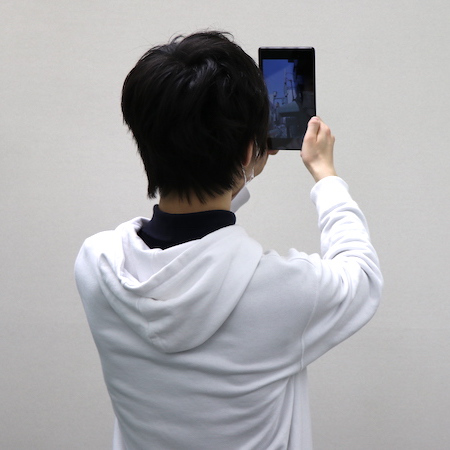
\includegraphics[width=\columnwidth, clip]{dr_exp.png}}
    \caption{実験風景(文献\cite{Kitamura:2017a}より図引用)}
    \label{figure:exp_dr_scenery}
  \end{figure}

  \begin{figure}[t]
    \begin{center}
      \begin{tabular}{cc}
        \begin{minipage}{0.45\hsize}
          \centering
          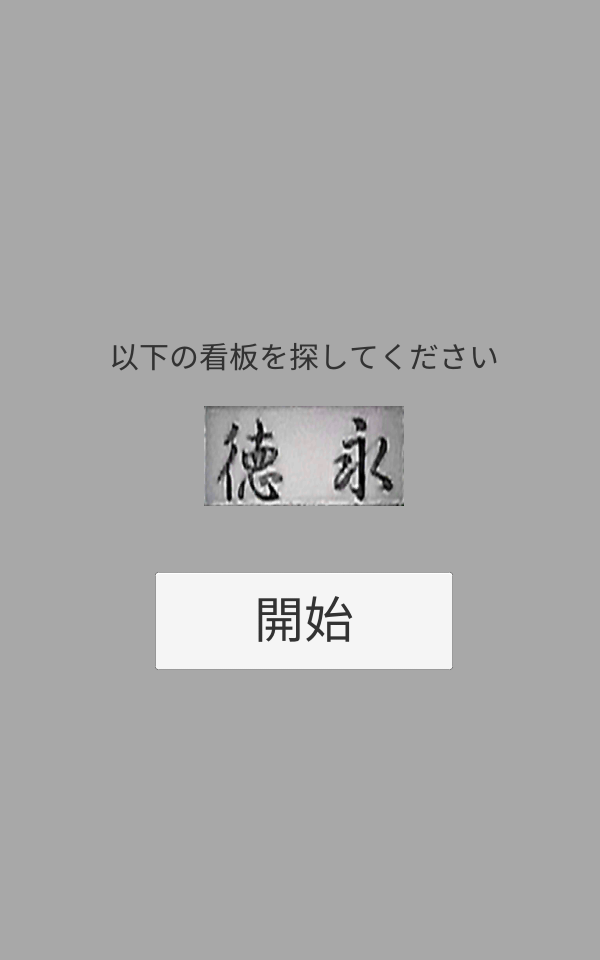
\includegraphics[clip, width=.9\textwidth]{dr_exp1.png}\\
          \small{(a)開始画面}
        \end{minipage}
        \begin{minipage}{0.45\hsize}
          \centering
          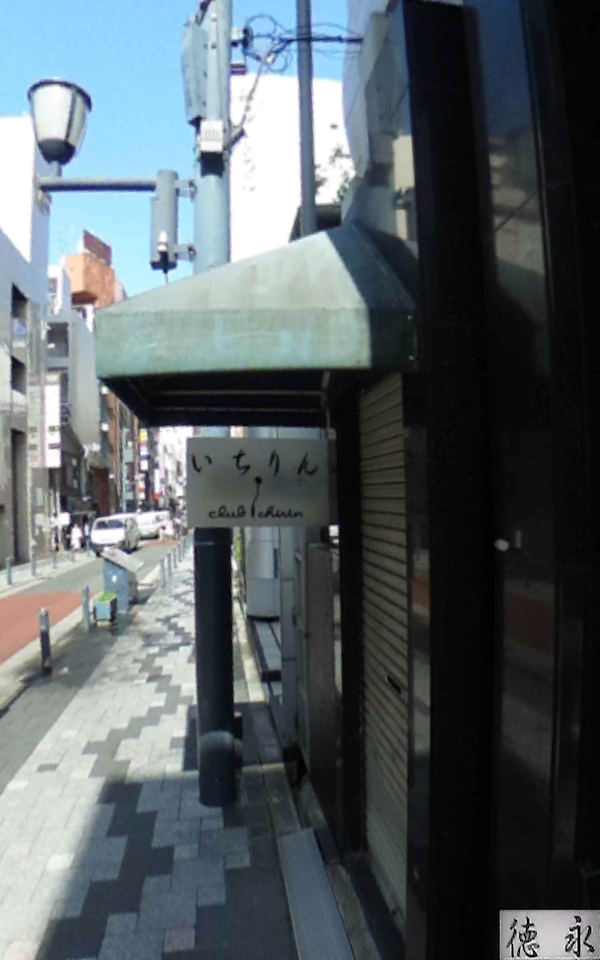
\includegraphics[clip, width=.9\textwidth]{dr_exp2.png}\\
          \small{(b)探索画面(1)}
        \end{minipage} \\\\
        \begin{minipage}{0.45\hsize}
          \centering
          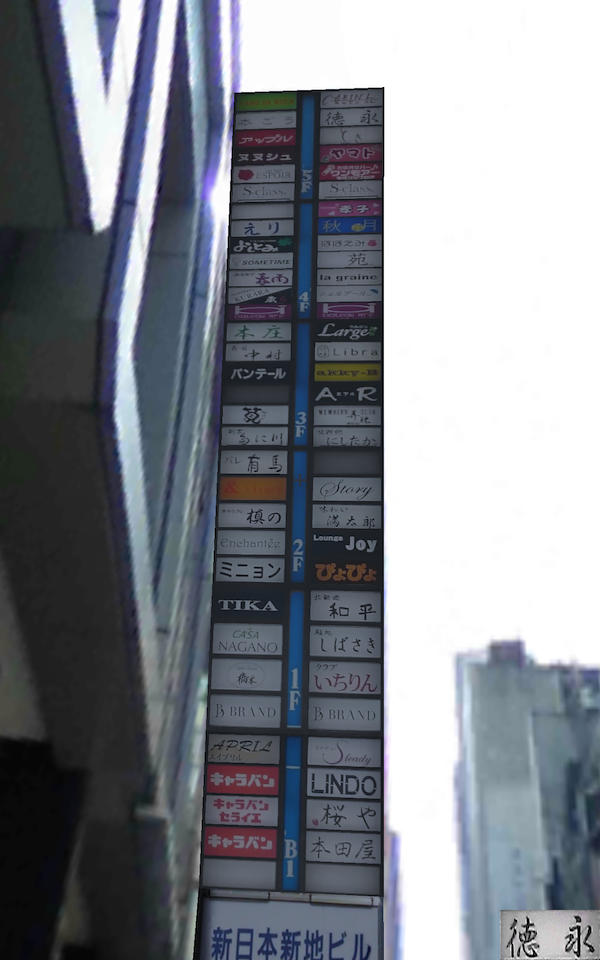
\includegraphics[clip, width=.9\textwidth]{dr_exp3.png}\\
          \small{(c)探索画面(2)}
        \end{minipage}
        \begin{minipage}{0.45\hsize}
          \centering
          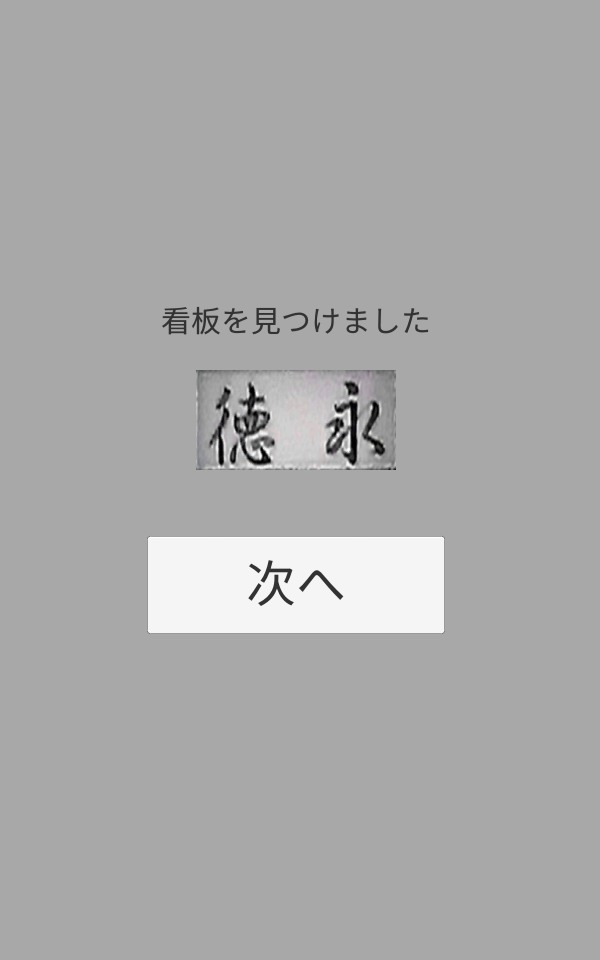
\includegraphics[clip, width=.9\textwidth]{dr_exp4.png}\\
          \small{(d)終了画面}
        \end{minipage}
      \end{tabular}
      \caption{実験の手順(文献\cite{Kitamura:2017a}より図引用)}
      \label{figure:exp_dr_procedure}
    \end{center}
  \end{figure}

\section{実験の結果}
  実験参加者が開始ボタンをタップしてから,指示された看板を全て見つけるまでの所要時間を計測し,通常型,加算型,減算型各々の探索時間とハイブリッド型の探索時間の平均値を比較した.その結果を以下に述べる.
  \subsection{時間帯が昼,探索対象が単体の場合}
    時間帯が昼,探索対象が単体の場合の探索時間を図\ref{figure:exp_dr_result_day} - (a) に示す.ハイブリッド型を用いた探索時間は,
    (1)通常型より有意に短い($t(22)=5.729, p<.05$)こと,
    (2)加算型より有意に短い($t(22)=2.852, p<.05$)ことが確認されたが,
    (3)減算型との間に有意差は見られなかった($t(22)=1.478, n.s.$).

  \subsection{時間帯が昼,探索対象が複数の場合}
    時間帯が昼,探索対象が複数の場合の探索時間を図\ref{figure:exp_dr_result_day} - (b) に示す.ハイブリッド型を用いた探索時間は,
    (1)通常型より有意に短い($t(22)=5.702, p<.05$)こと,
    (2)加算型より有意に短い($t(22)=6.144, p<.05$)こと,
    (3)減算型より有意に短い($t(22)=3.318, p<.05$)ことがそれぞれ確認された.

  \subsection{時間帯が夜,探索対象が単体の場合}
    時間帯が夜,探索対象が単体の場合の探索時間を図\ref{figure:exp_dr_result_night} - (a) に示す.ハイブリッド型を用いた探索時間は,
    (1)通常型より有意に短い($t(22)=4.325, p<.05$)こと,
    (2)加算型より有意に短い($t(22)=2.103, p<.05$)こと,
    (3)減算型より有意に短い($t(22)=2.485, p<.05$)ことがそれぞれ確認された.

  \subsection{時間帯が夜,探索対象が複数の場合}
    時間帯が夜,探索対象が複数の場合の探索時間を図\ref{figure:exp_dr_result_night} - (b) に示す.ハイブリッド型を用いた探索時間は,
    (1)通常型より有意に短い($t(22)=5.512, p<.05$)こと,
    (2)加算型との間に有意差はない($t(22)=1.857, n.s.$)こと,
    (3)減算型より有意に短い($t(22)=3.129, p<.05$)ことがそれぞれ確認された.

  \subsection{アンケート結果}
    実験終了後に,最も対象の看板を見つけやすかった提示手法についてアンケートを実施したところ,実験参加者の過半数が提案手法であるハイブリッド型情報提示手法を選択した.

  \begin{figure}[t]
    \begin{center}
      \begin{tabular}{cc}
        \begin{minipage}{0.45\hsize}
          \centering
          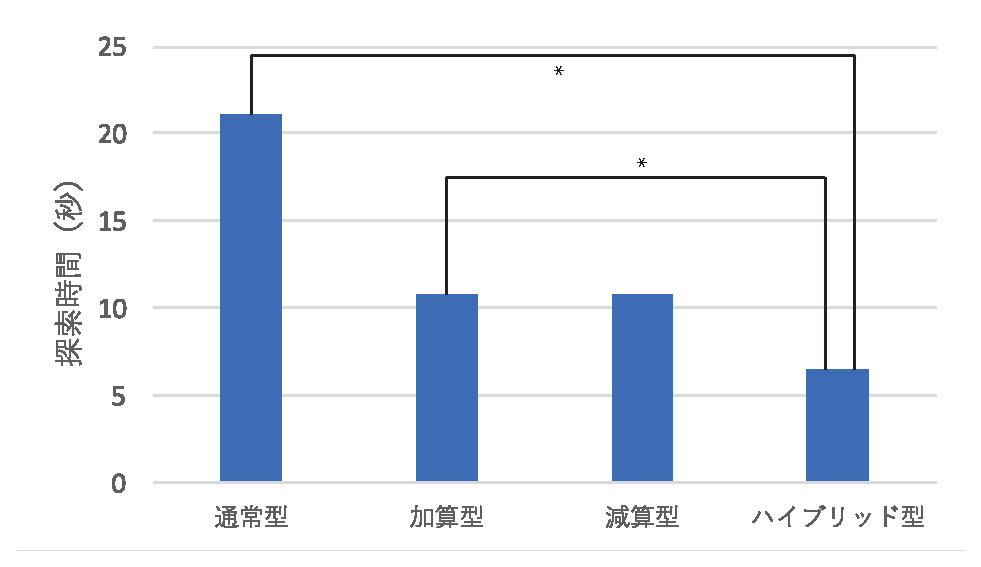
\includegraphics[clip, width=.95\textwidth]{dr_result1.eps}\\
          \small{(a)対象:単体}
        \end{minipage}
        \begin{minipage}{0.45\hsize}
          \centering
          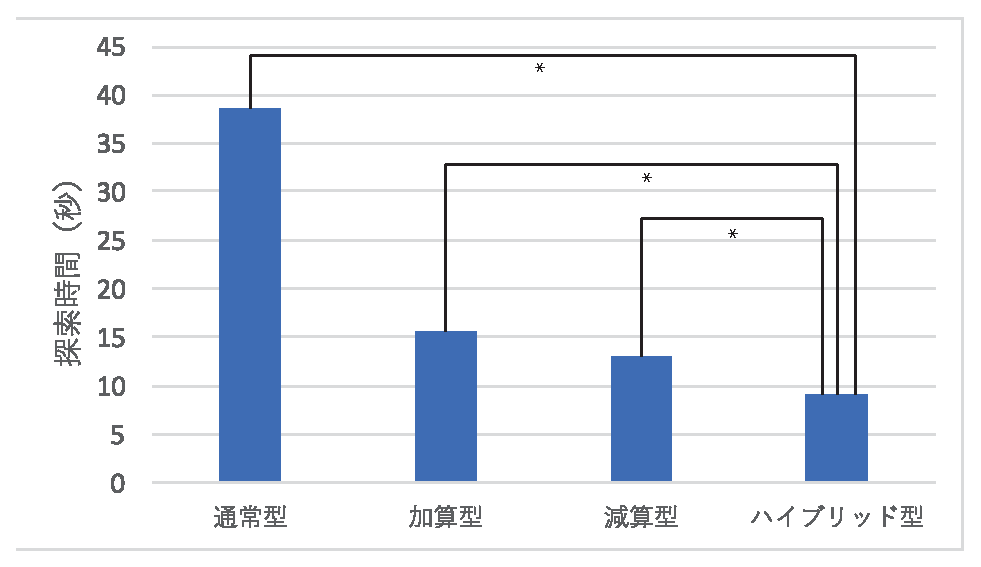
\includegraphics[clip, width=.95\textwidth]{dr_result2.eps}\\
          \small{(b)対象:複数}
        \end{minipage}
      \end{tabular}
      \vspace{2pt}
      \caption{実験結果:昼($*:p<.05$)(文献\cite{Kitamura:2017a}より図引用)}
      \label{figure:exp_dr_result_day}
      \vspace{2cm}
      \begin{tabular}{cc}
        \begin{minipage}{0.45\hsize}
          \centering
          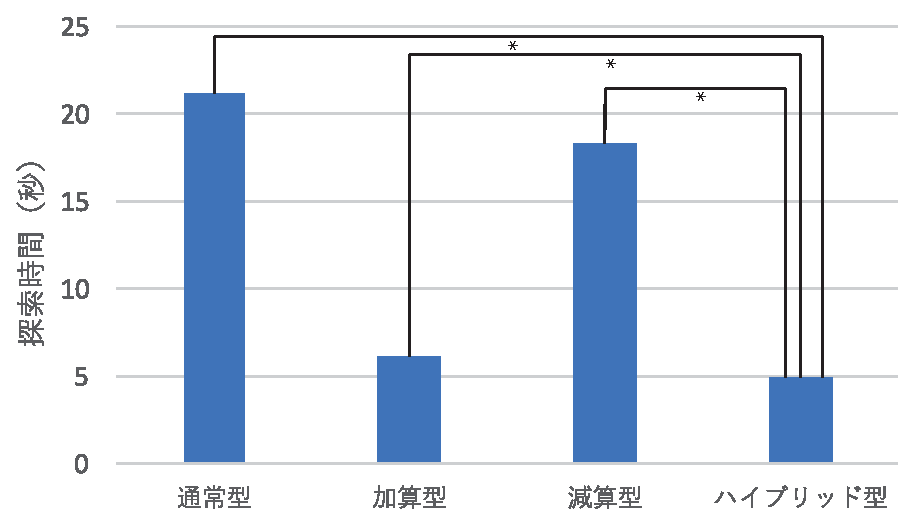
\includegraphics[clip, width=.95\textwidth]{dr_result3.eps}\\
          \small{(a)対象:単体}
        \end{minipage}
        \begin{minipage}{0.45\hsize}
          \centering
          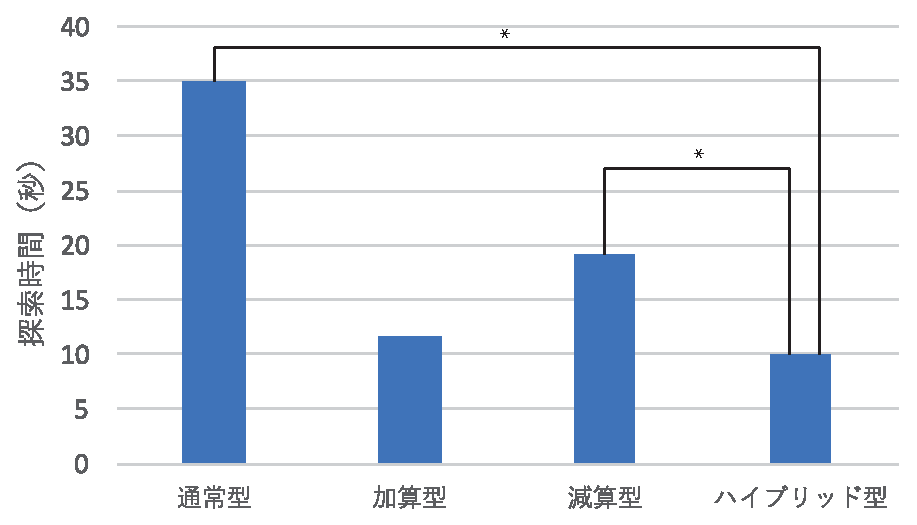
\includegraphics[clip, width=.95\textwidth]{dr_result4.eps}\\
          \small{(b)対象:複数}
        \end{minipage}
      \end{tabular}
      \vspace{2pt}
      \caption{実験結果:夜($*:p<.05$)(文献\cite{Kitamura:2017a}より図引用)}
      \label{figure:exp_dr_result_night}
    \end{center}
  \end{figure}